% Midterm Report

% Your milestone report should be 1 - 2 (max) pages and answer the following questions:
% 1. What has been done so far? (tools decided on, implementations, overview on methods, …)
% 2. First Results (e.g., some raw plots)
% (no explicit introduction, because you described your topic already in the proposal)

% The milestone report must report on at least one experiment that you have done since the proposal. This experiment does not need to be successful, but you should have attempted something. If it did not work as expected, you should briefly discuss why. You are encouraged to include a plot or figure.

% The format for the report has to be the standard IEEE conference format: https://www.ieee.org/conferences/publishing/templates.html

\documentclass[conference]{IEEEtran}
\usepackage{cite}
\usepackage{amsmath,amssymb,amsfonts}
\usepackage{algorithmic}
\usepackage{graphicx}
\usepackage{textcomp}
\usepackage{xcolor}

% \usepackage{subcaption}
% \captionsetup{compatibility=false}

\ifCLASSOPTIONcompsoc
\usepackage[caption=false,font=normalsize,labelfont=sf,textfont=sf{subfig}
\else
\usepackage[caption=false,font=footnotesize]{subfig}

\fi
\def\BibTeX{{\rm B\kern-.05em{\sc i\kern-.025em b}\kern-.08emT\kern-.1667em\lower.7ex\hbox{E}\kern-.125emX}}

\begin{document}


\title{Milestone Report}

\author{\IEEEauthorblockN{Franziska Schwaiger}
    \IEEEauthorblockA{\textit{Matriculation number: 03658670}}
    \and
    \IEEEauthorblockN{Thomas Brunner}
    \IEEEauthorblockA{\textit{Matriculation number: 03675118}}
}

\maketitle

\section*{Dataset}

\begin{figure*}[t]
    \centering
    \subfloat[2 DOF]{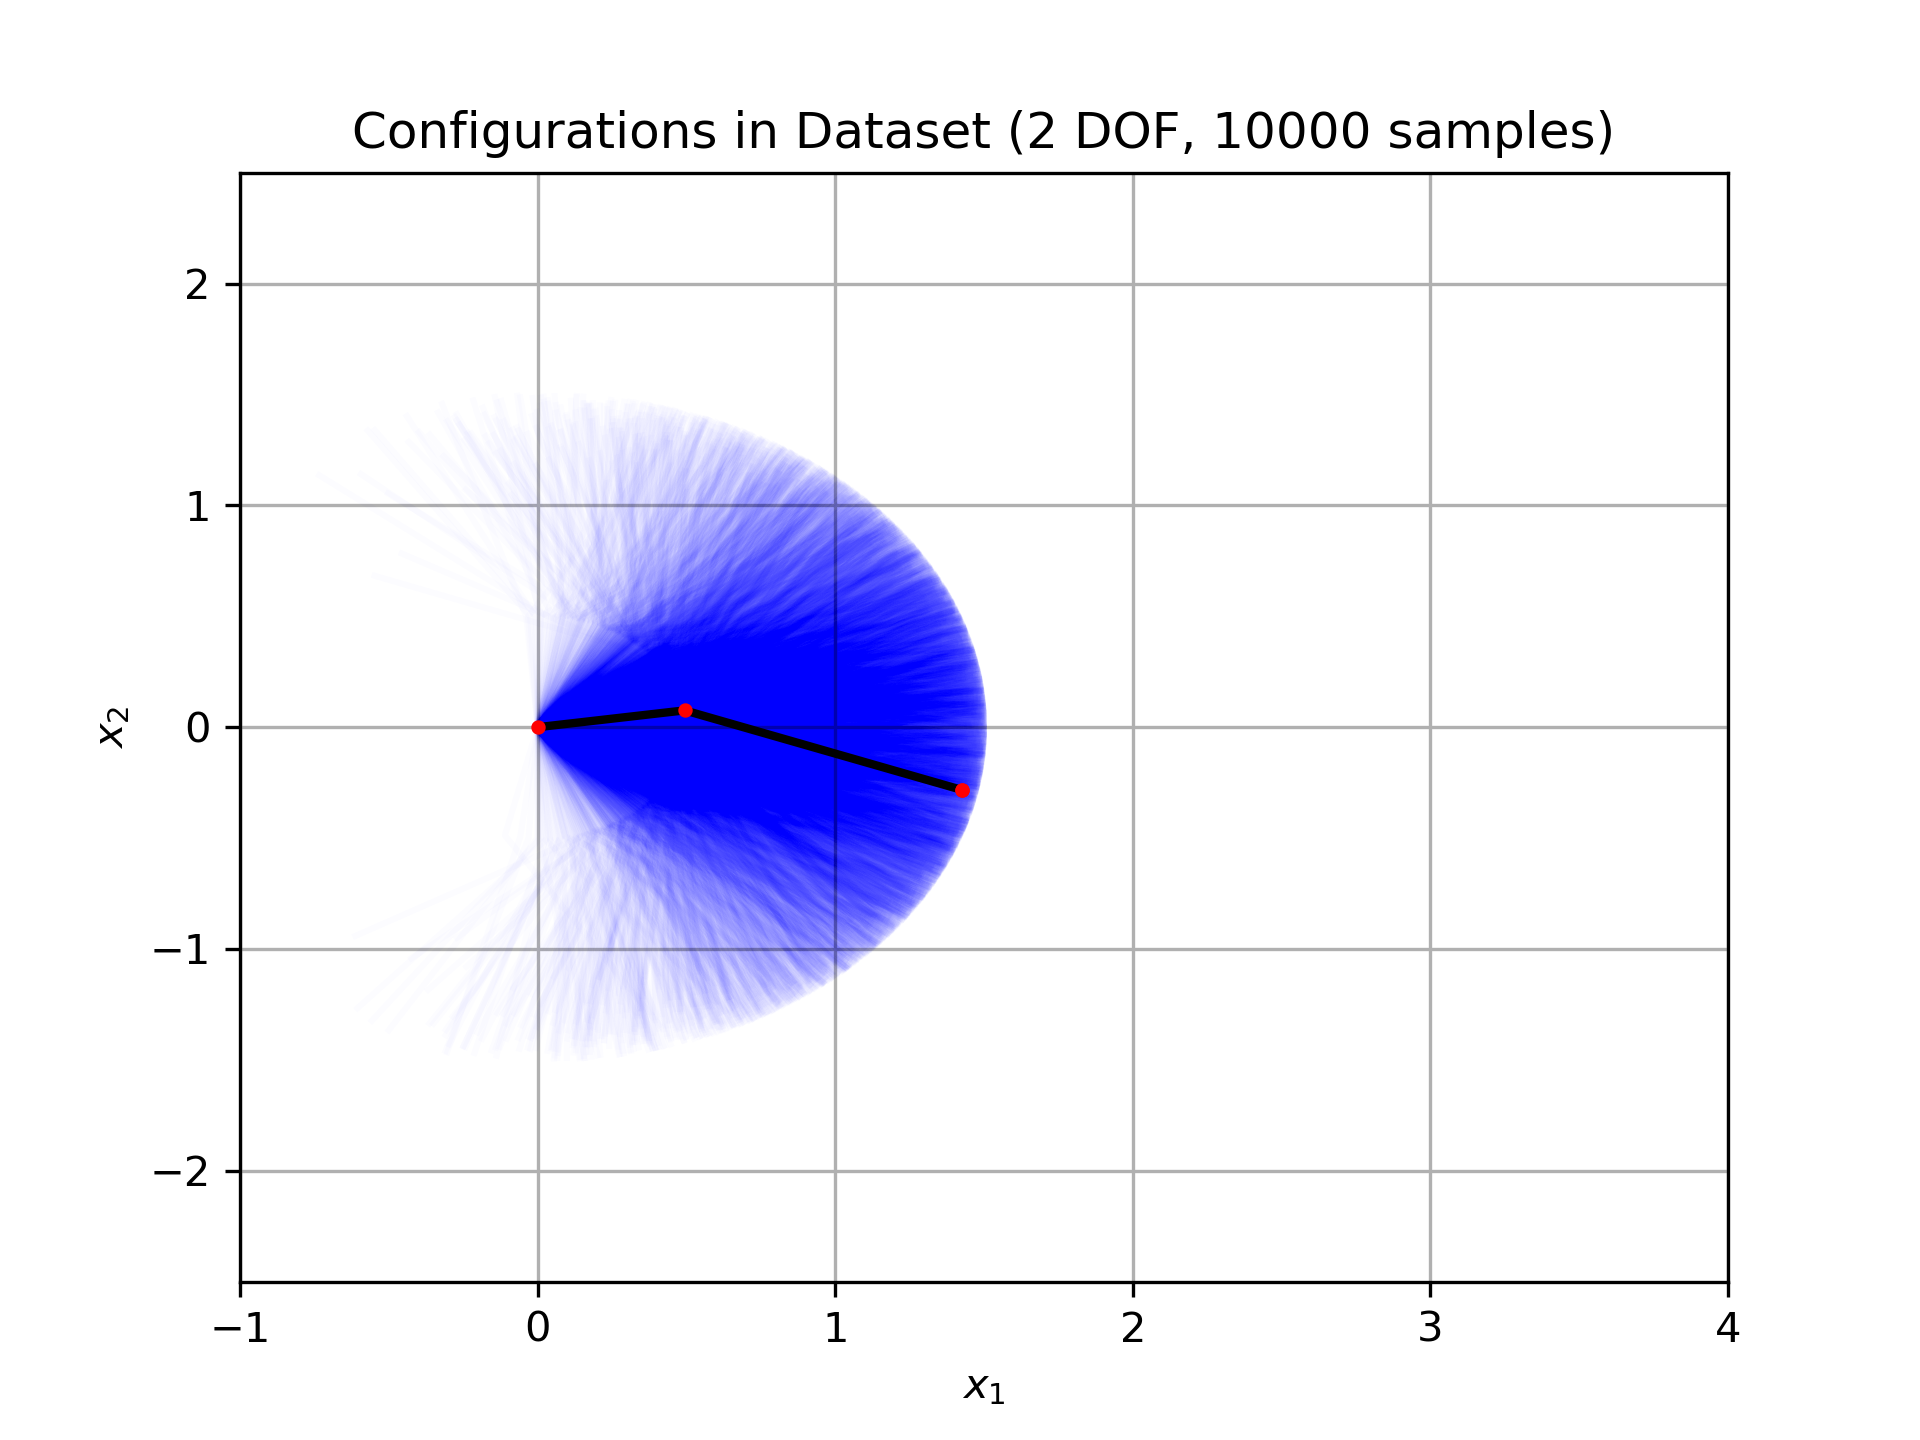
\includegraphics[width=0.3\linewidth]{figures/normal_2dof_configs.png}
        \label{fig_first_case}}
    \subfloat[3 DOF]{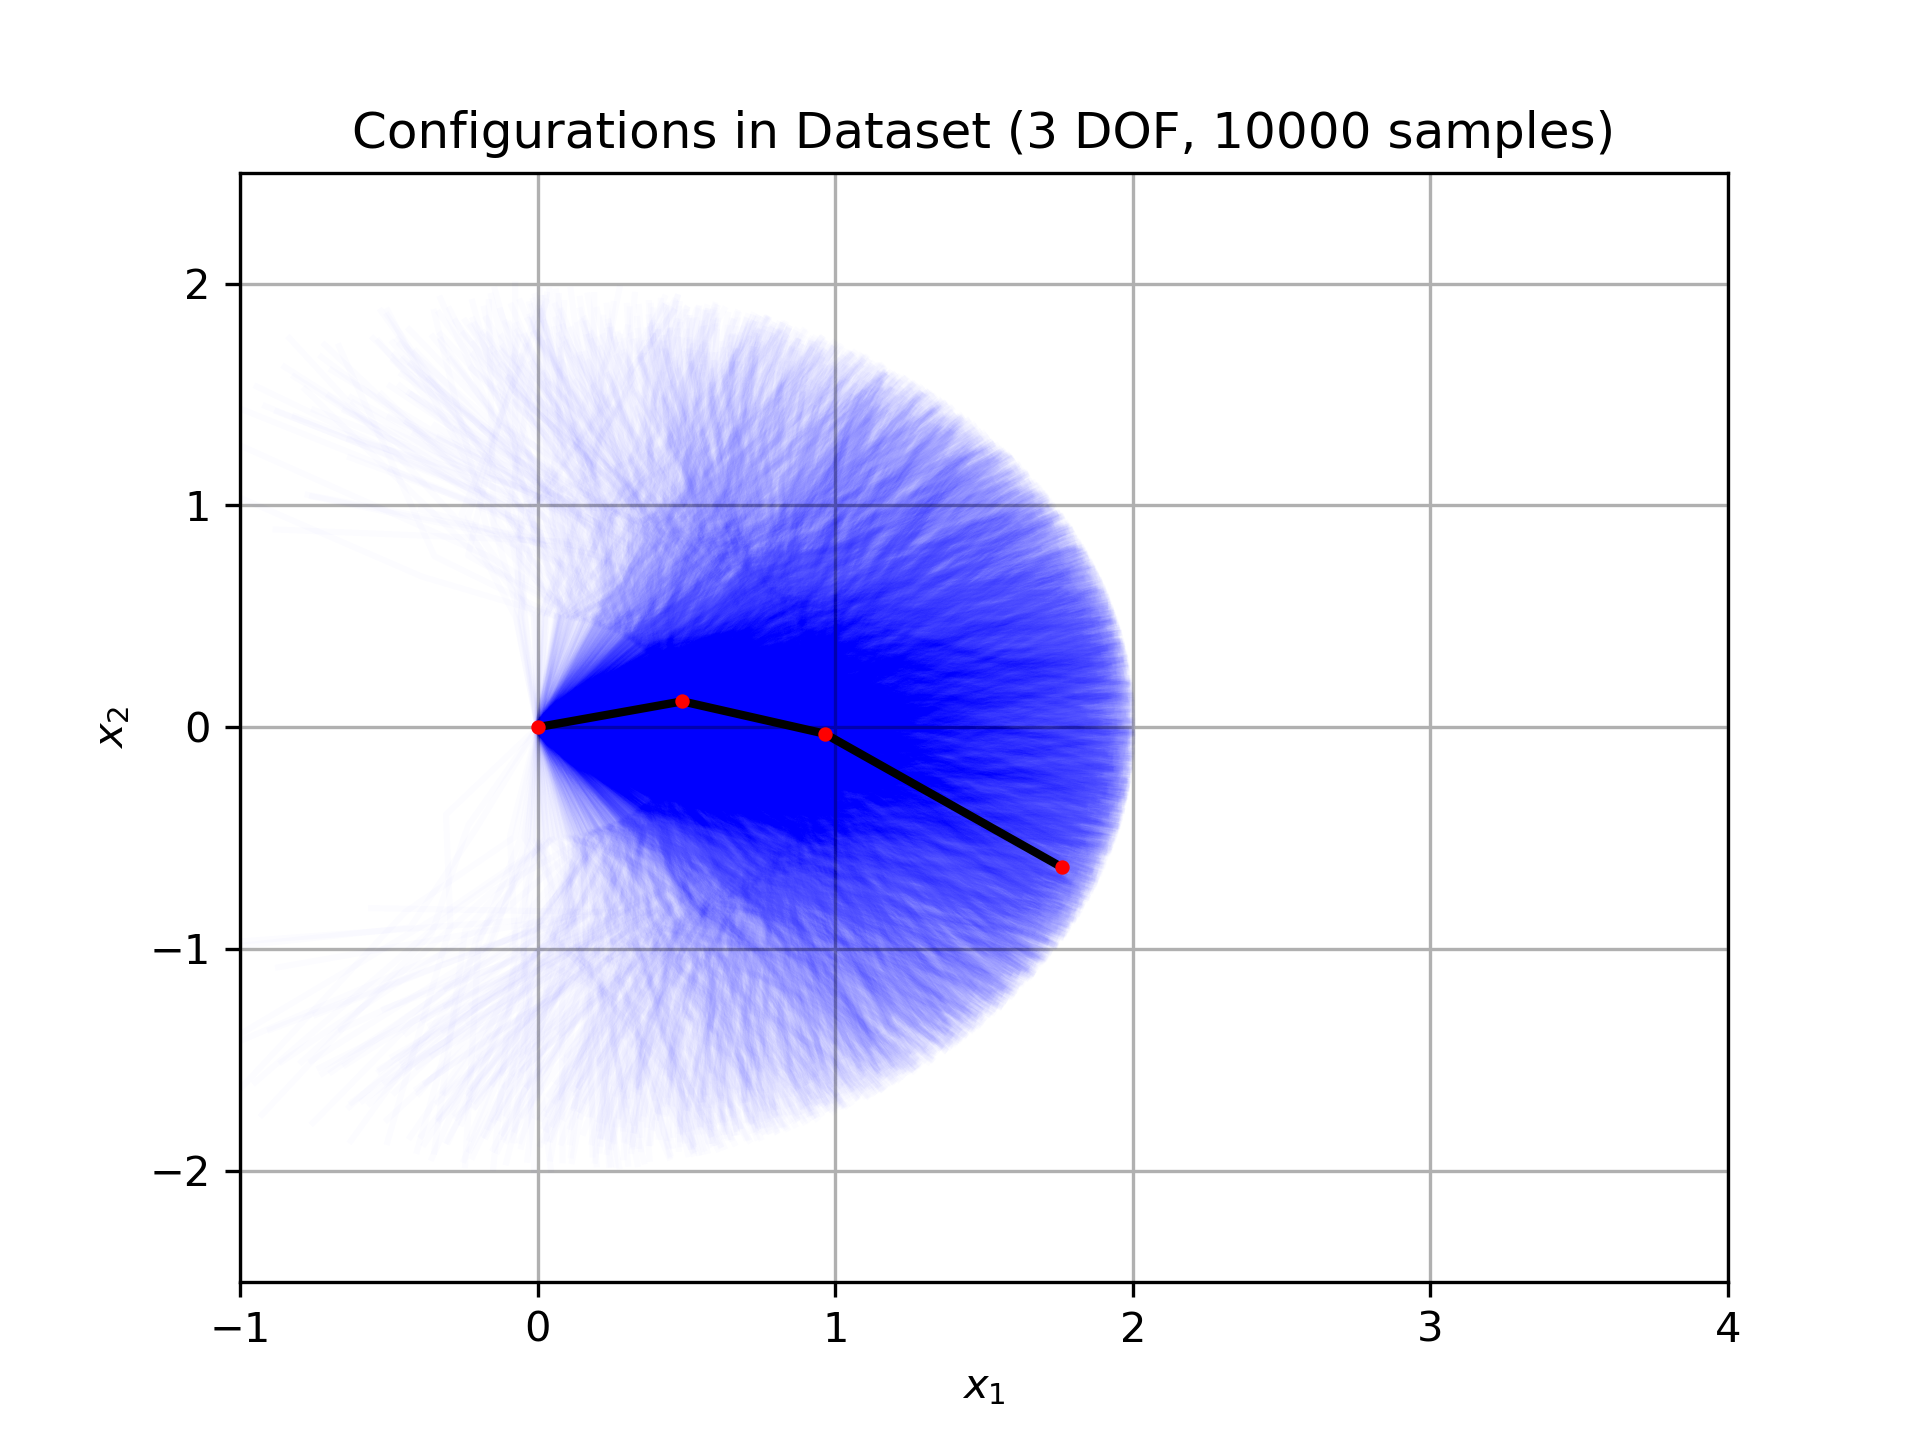
\includegraphics[width=0.3\linewidth]{figures/normal_3dof_configs.png}
        \label{fig_second_case}}
    \subfloat[4 DOF]{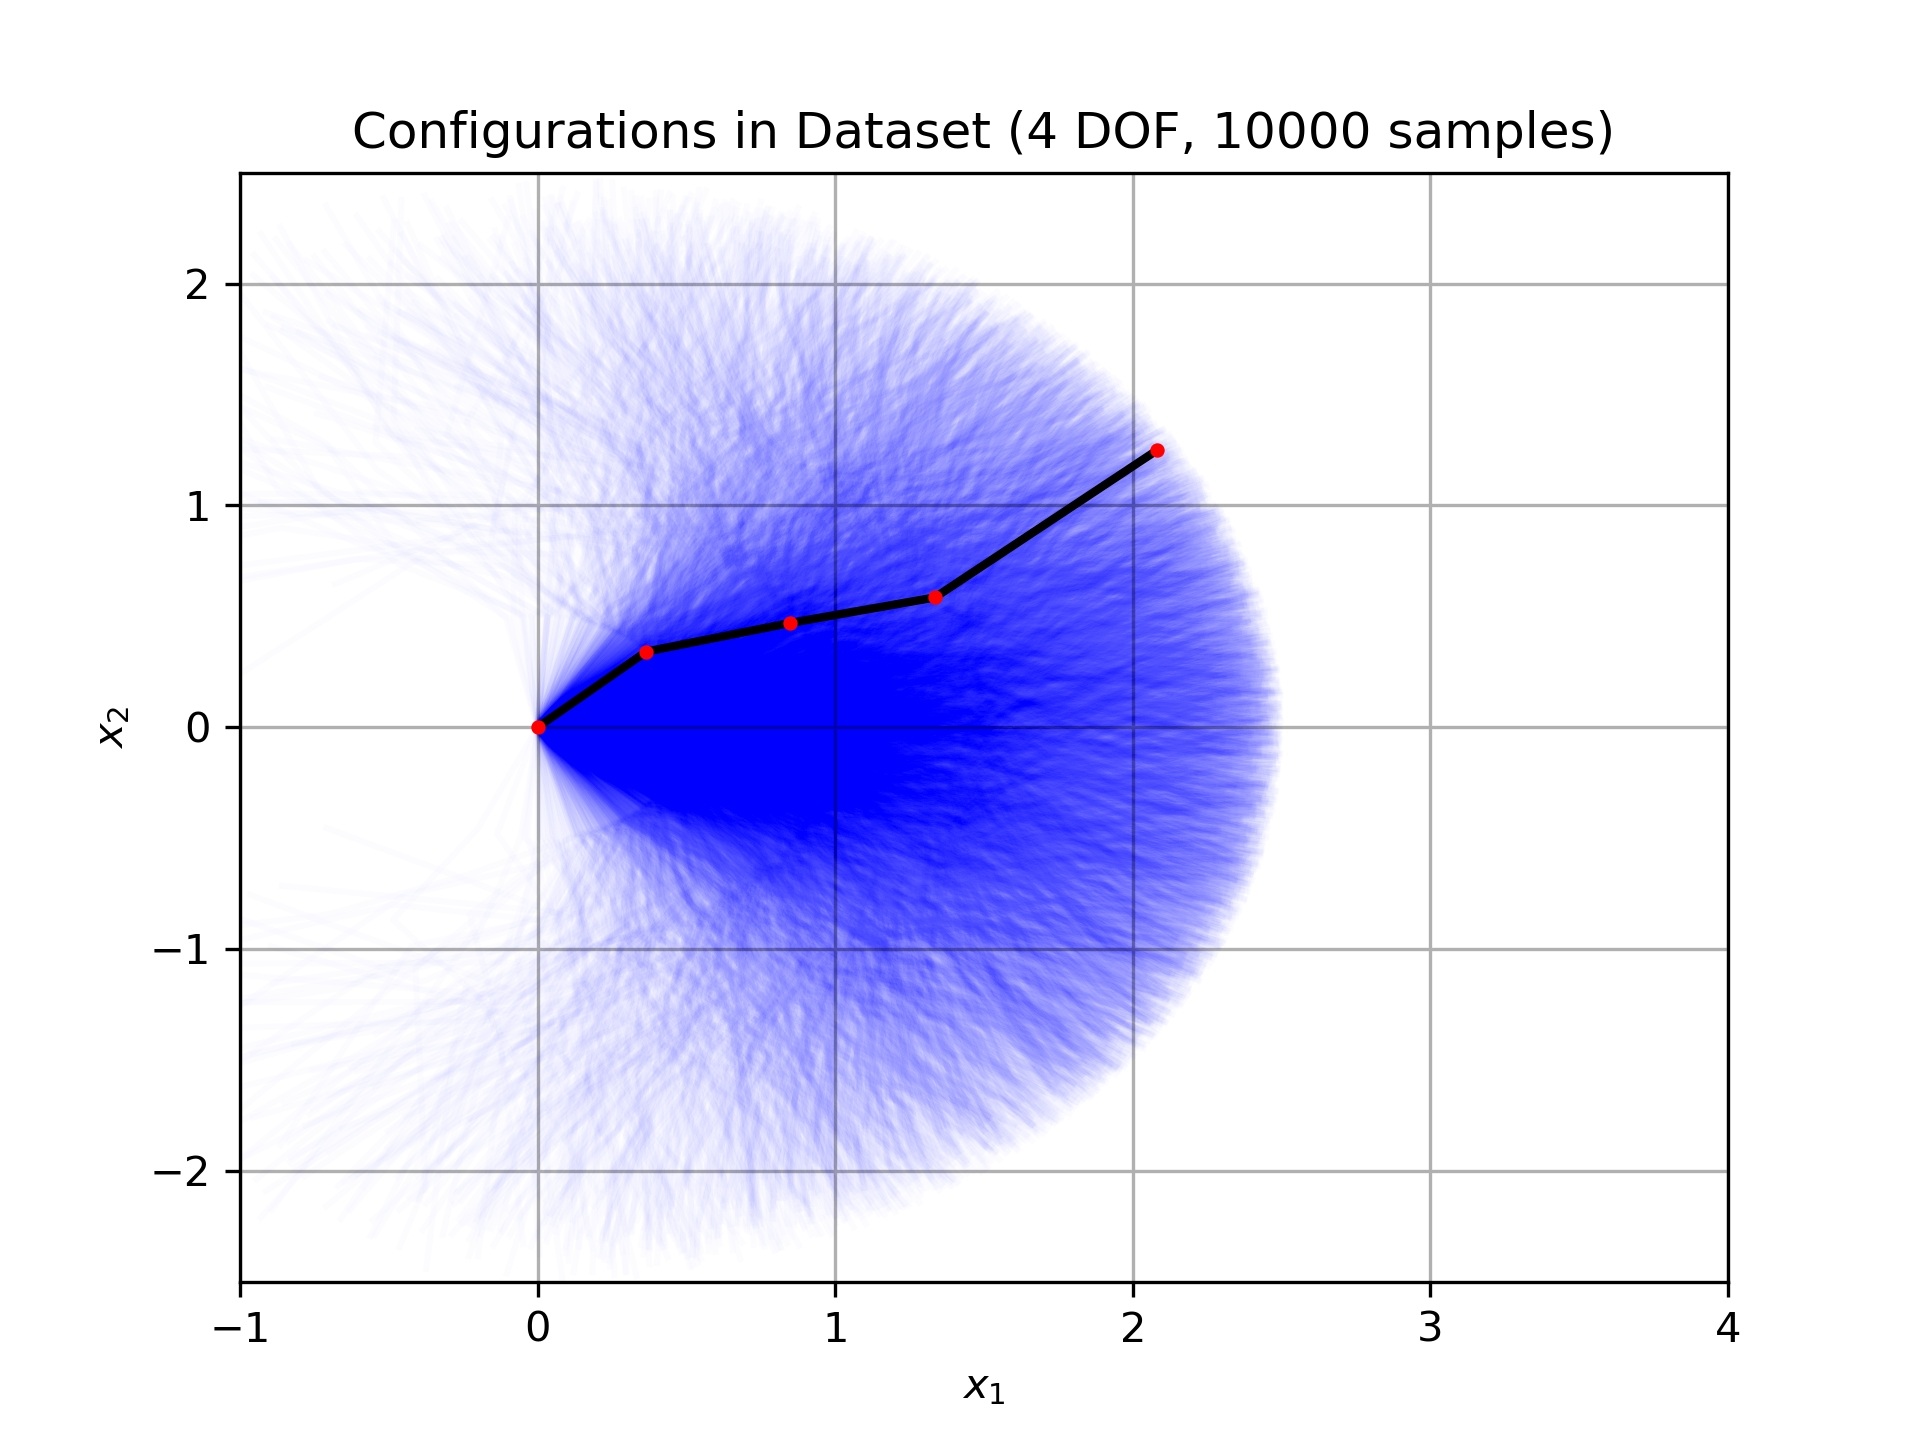
\includegraphics[width=0.3\linewidth]{figures/normal_4dof_configs.png}
        \label{fig_second_case}}
    \caption{Illustration of datasets used during training of models. Only a subset of the samples contained in the datasets is shown here. One configuration in the dataset is highlighted to illustrate the configuration of the robot arm.}
    \label{fig_sim}
\end{figure*}


\section*{Methods}

The following two model architectures have been implemented in PyTorch and are inspired by GitHub repositories \cite{graviraja2019}, \cite{freia2020}.

\subsection*{Conditional Variational Autoencoder}

In the lecture, we have already discussed Variational Autoencoders (VAE) \cite{Kingma2014} in detail. One drawback of this type of generative architecture is that there is no control over the data generation process. In our case this would mean that although we can generate random sample configurations we cannot control in which end-effector position these configurations would result. Conditional Variational Autoencoders (cVAE) \cite{Sohn2015} solve this problem by conditioning the latent space $z$. For inverse kinematics this means that random samples are drawn from $p(z) \sim N(0, 1)$ and the predicted posterior of the joint angles is then generated conditioned on the end-effector position. During training, the position $(x, y)$ is concatenated with both $x$ and $z$ and then fed into the encoder and decoder, respectively.

The cVAE is trained in the same manner as the VAE based on the ELBO (Evidence Lower Bound) loss $L_{ELBO} = L_y + L_x$: 

\begin{equation}
L_y = - KL[q_\phi(z | x, y) || p(z) \sim N(0, 1) ]
\label{ELBO}
\end{equation}

The Kullback-Leibler divergence measures the distance between the predicted probability distribution $q_\phi(z | x, y)$ of the latent space $z$ and the standard normal distribution. The reconstruction loss is defined as follows: 

\begin{equation}
L_x = E_{q_\phi(z | x)}[log(p_\theta(x| z, y))] = \sum _ {i=0} ^ N MSE(v_i \cdot \tilde v_i, 1)
\label{MSE}
\end{equation}

Here, $N$ is denoted as the  number of joints. For representing the joint angles of the robot, we use a vector-based representation: $V = (sin(\theta), cos(\theta))$ to avoid singularities at the boundaries of the joint angles. $v_i \cdot \tilde v_i$ is denoted as the scalar product between the normalized predicted posterior point estimate  $\tilde v_i  = (sin(\tilde \theta), cos(\tilde \theta))$ and the ground truth vector  $v_i = (sin(\theta), cos(\theta))$ of the ith joint.

\subsection*{Invertible Neural Network}

\section*{Experimental Evaluation}

\subsection*{Evaluation protocol}
\subsection*{Results}

\begin{table}[h]
\centering
\begin{tabular}{|c|c|c|c|c|}
\hline
 DoF & $e_{posterior}$ & $e_{resim}$ & Trainable Parameters & Model \\
 \hline
 2  & 0.077 & \textbf{0.003} & 164,808 & \\
 3  & \textbf{0.045} & 0.045 & 370,214 & cVAE \\
 4  & 0.063 & \textbf{0.006} & 373,220 & \\
 \hline
 2  & \textbf{0.061} & 0.012 & 169,632 & \\
 3  & 0.066 & \textbf{0.036} & 369,660 & INN \\
 4  & \textbf{0.044} & 0.075 & 374,960 & \\
 \hline
\end{tabular}
\caption{\label{tab:results} Caption to come}
\end{table}

\begin{figure*}[t]
\centering
	\subfloat[Rejection Sampling]{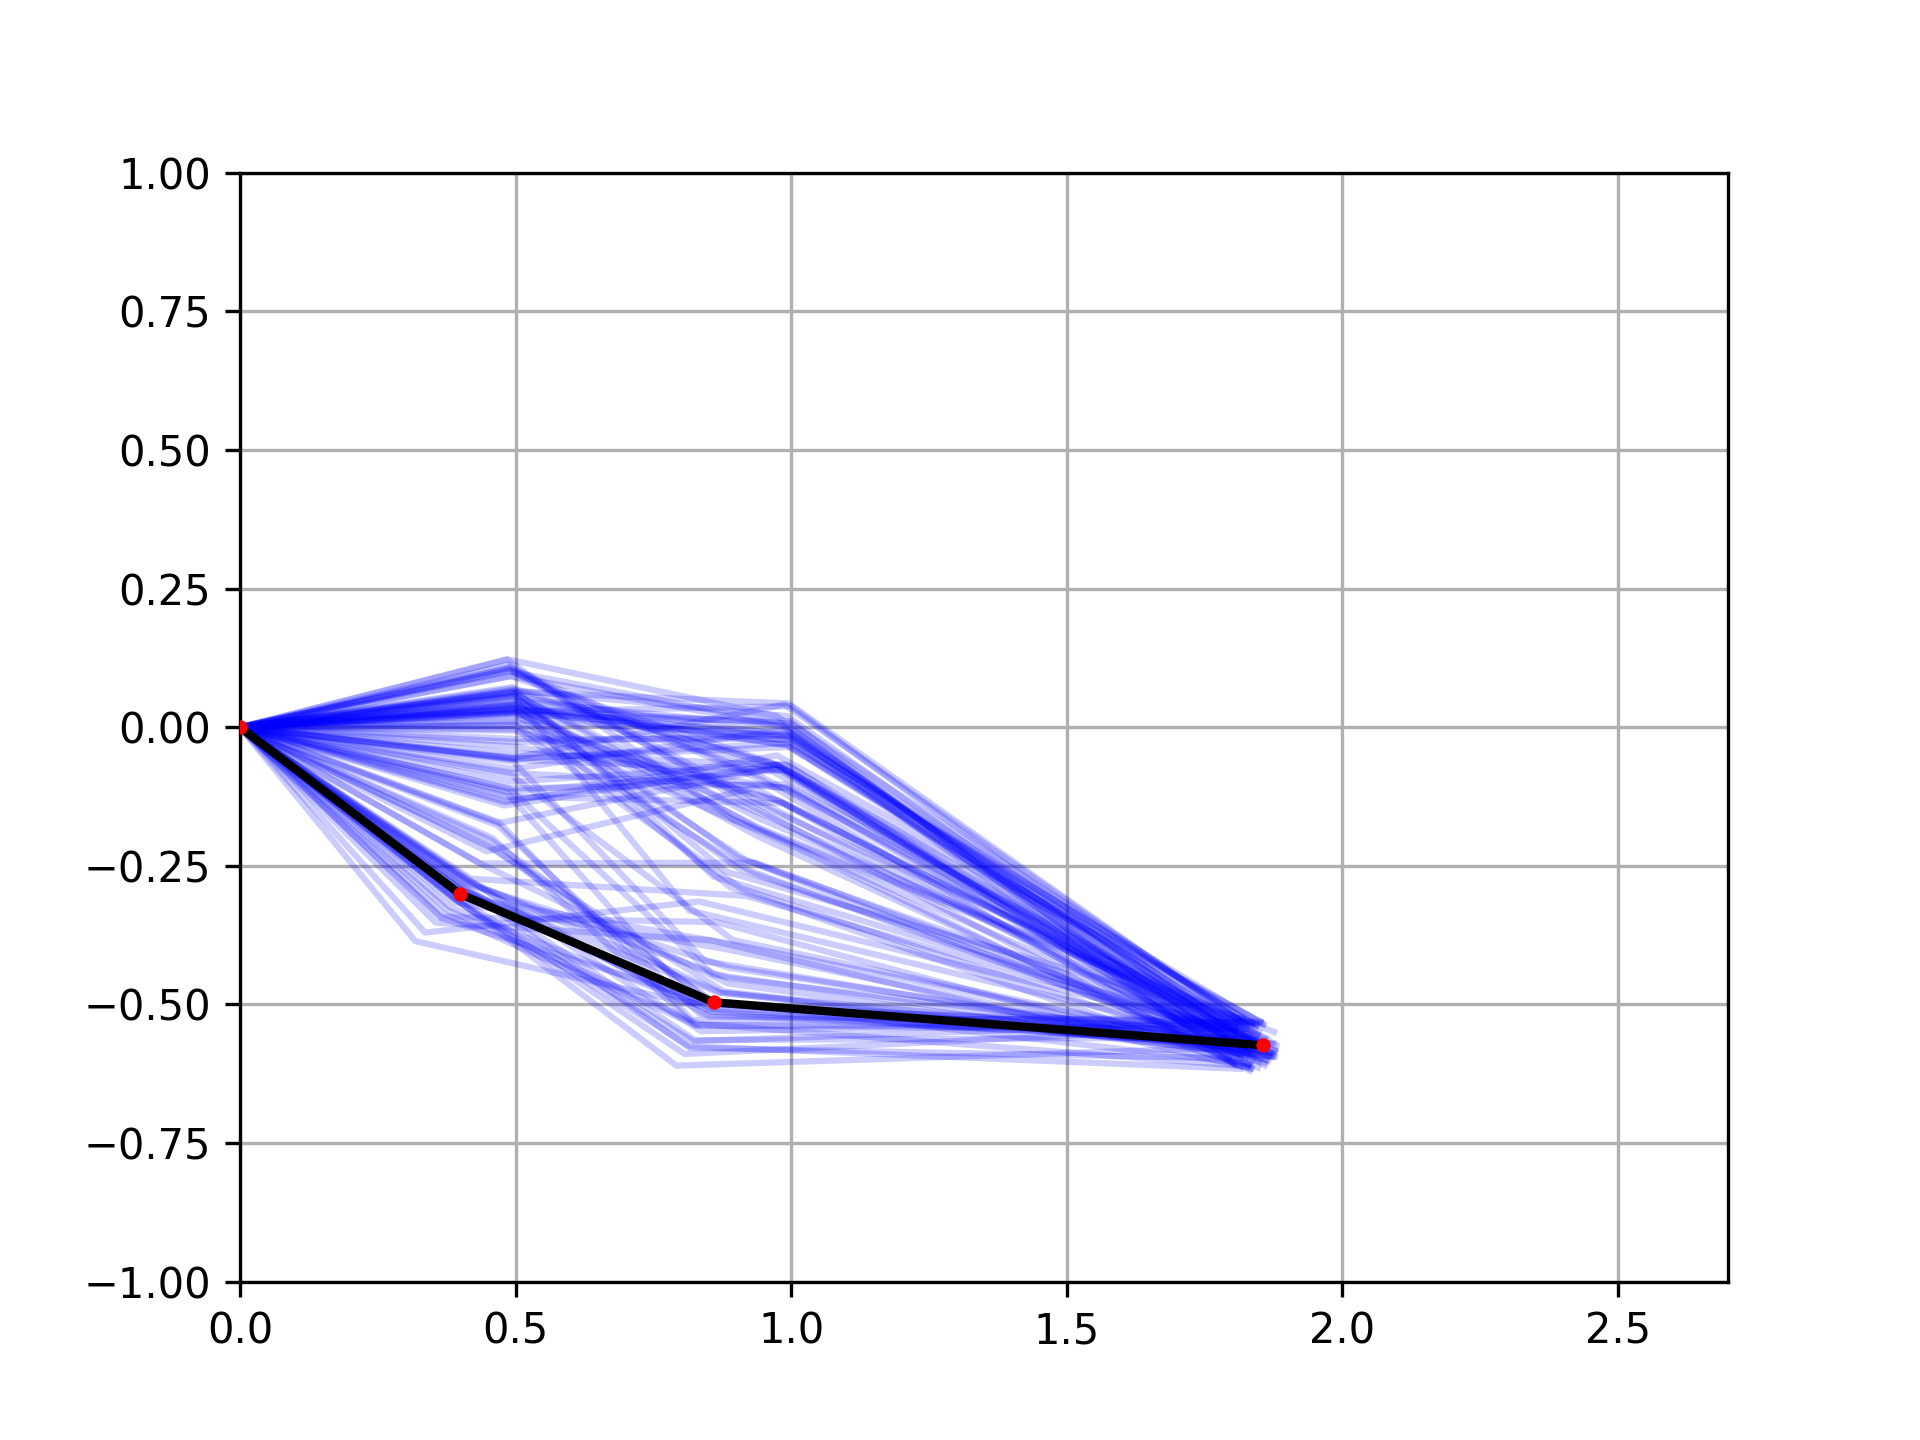
\includegraphics[width=0.29\linewidth]{figures/rejection_sampling_INN_3DOF.png}
    \label{fig:rejection_sampling:3DOF}}
    %
    \subfloat[cVAE]{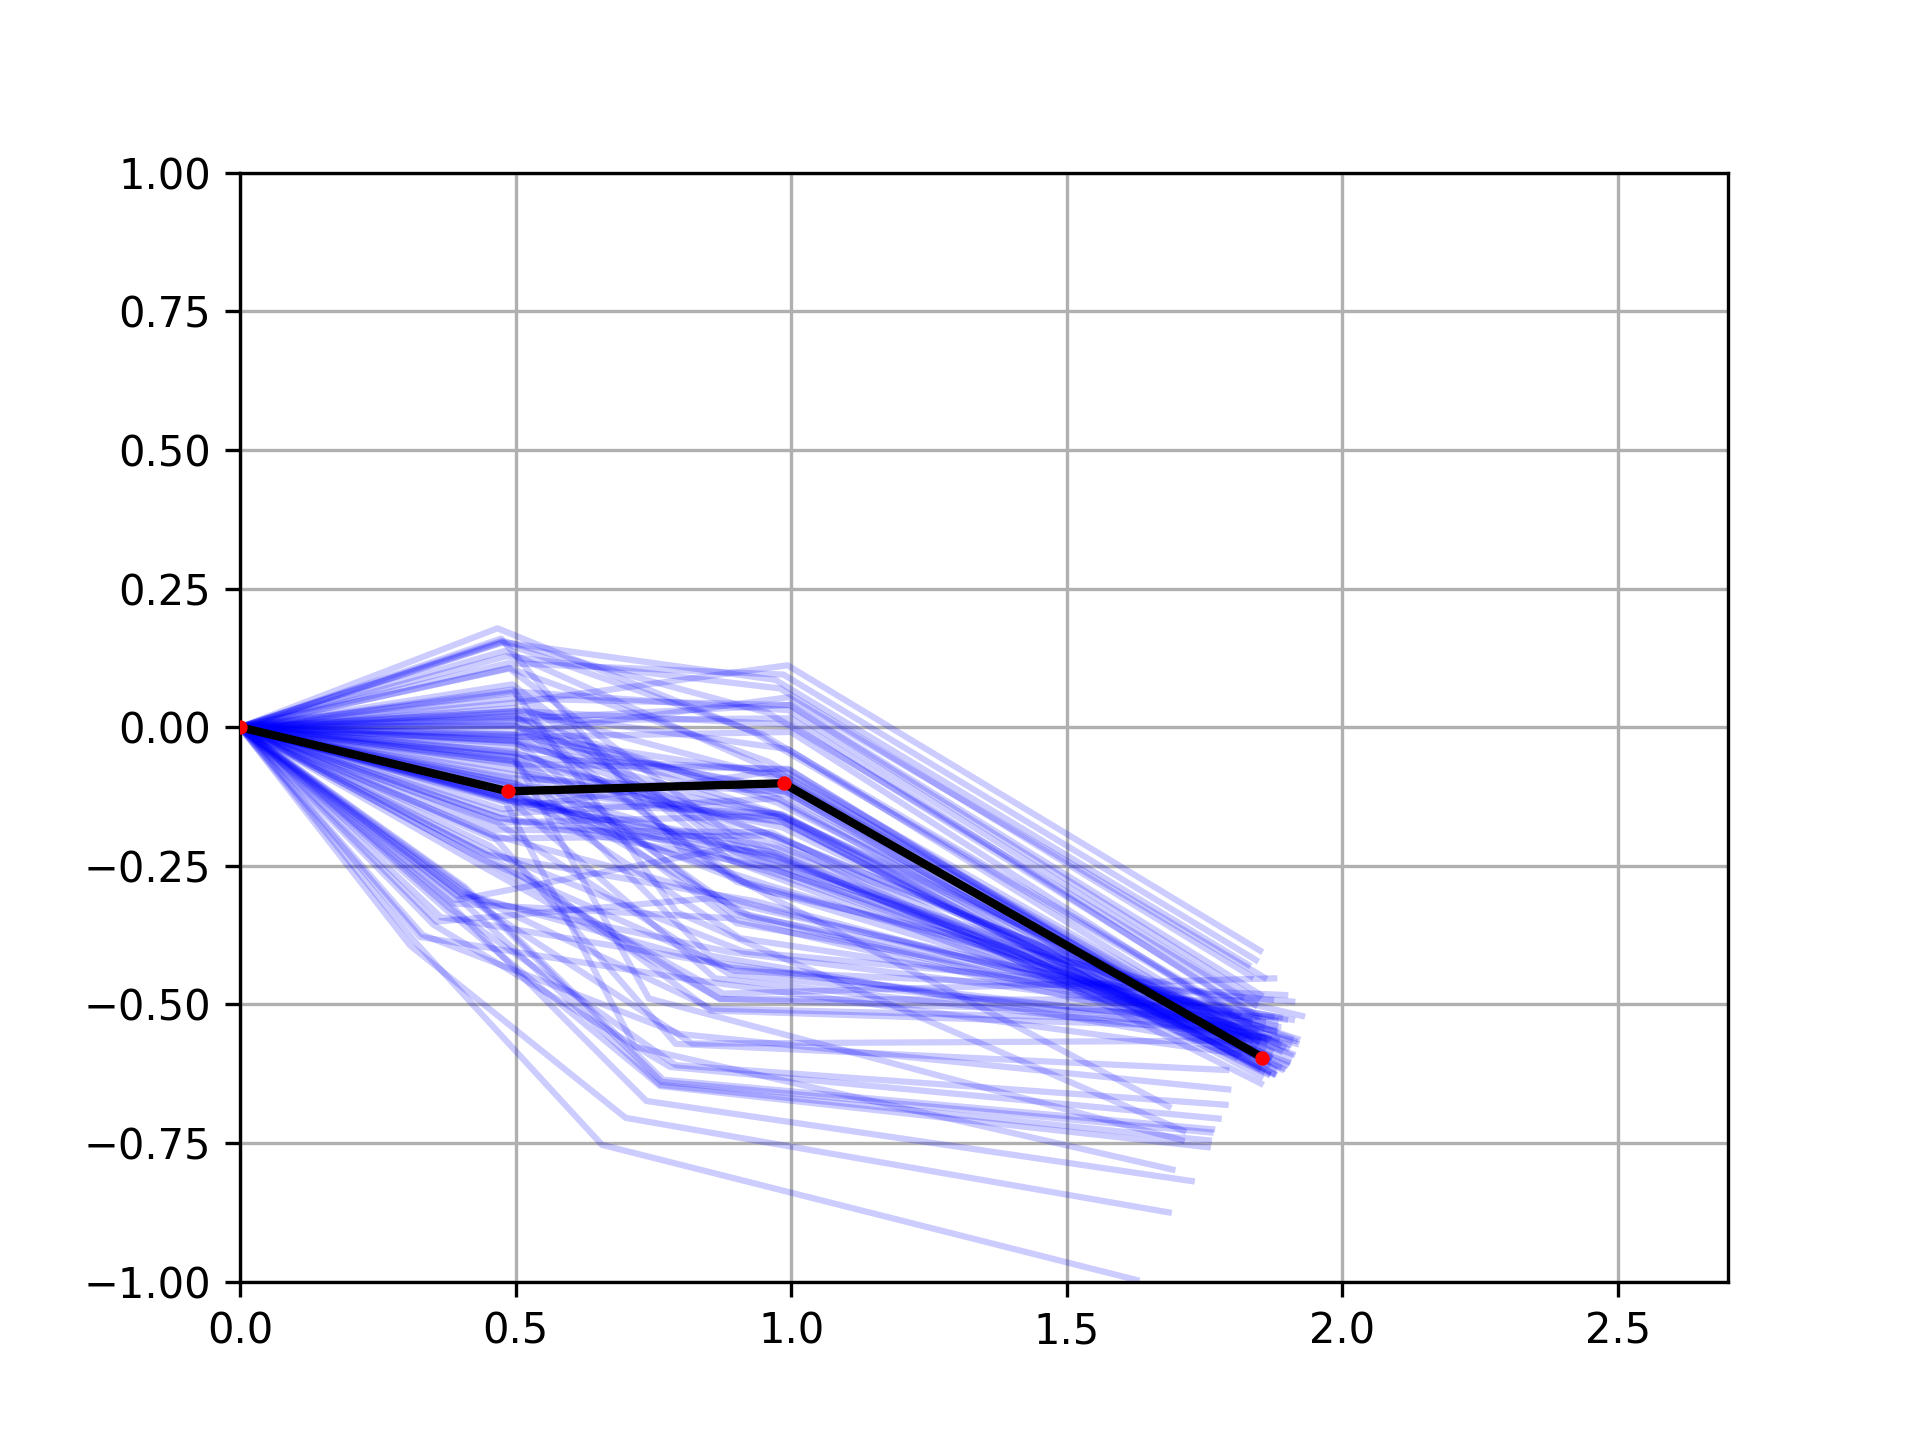
\includegraphics[width=0.29\linewidth]{figures/predicted_posterior_CVAE_3DOF.png}
    \label{fig:cVAE:3DOF}}
    %
    \subfloat[INN]{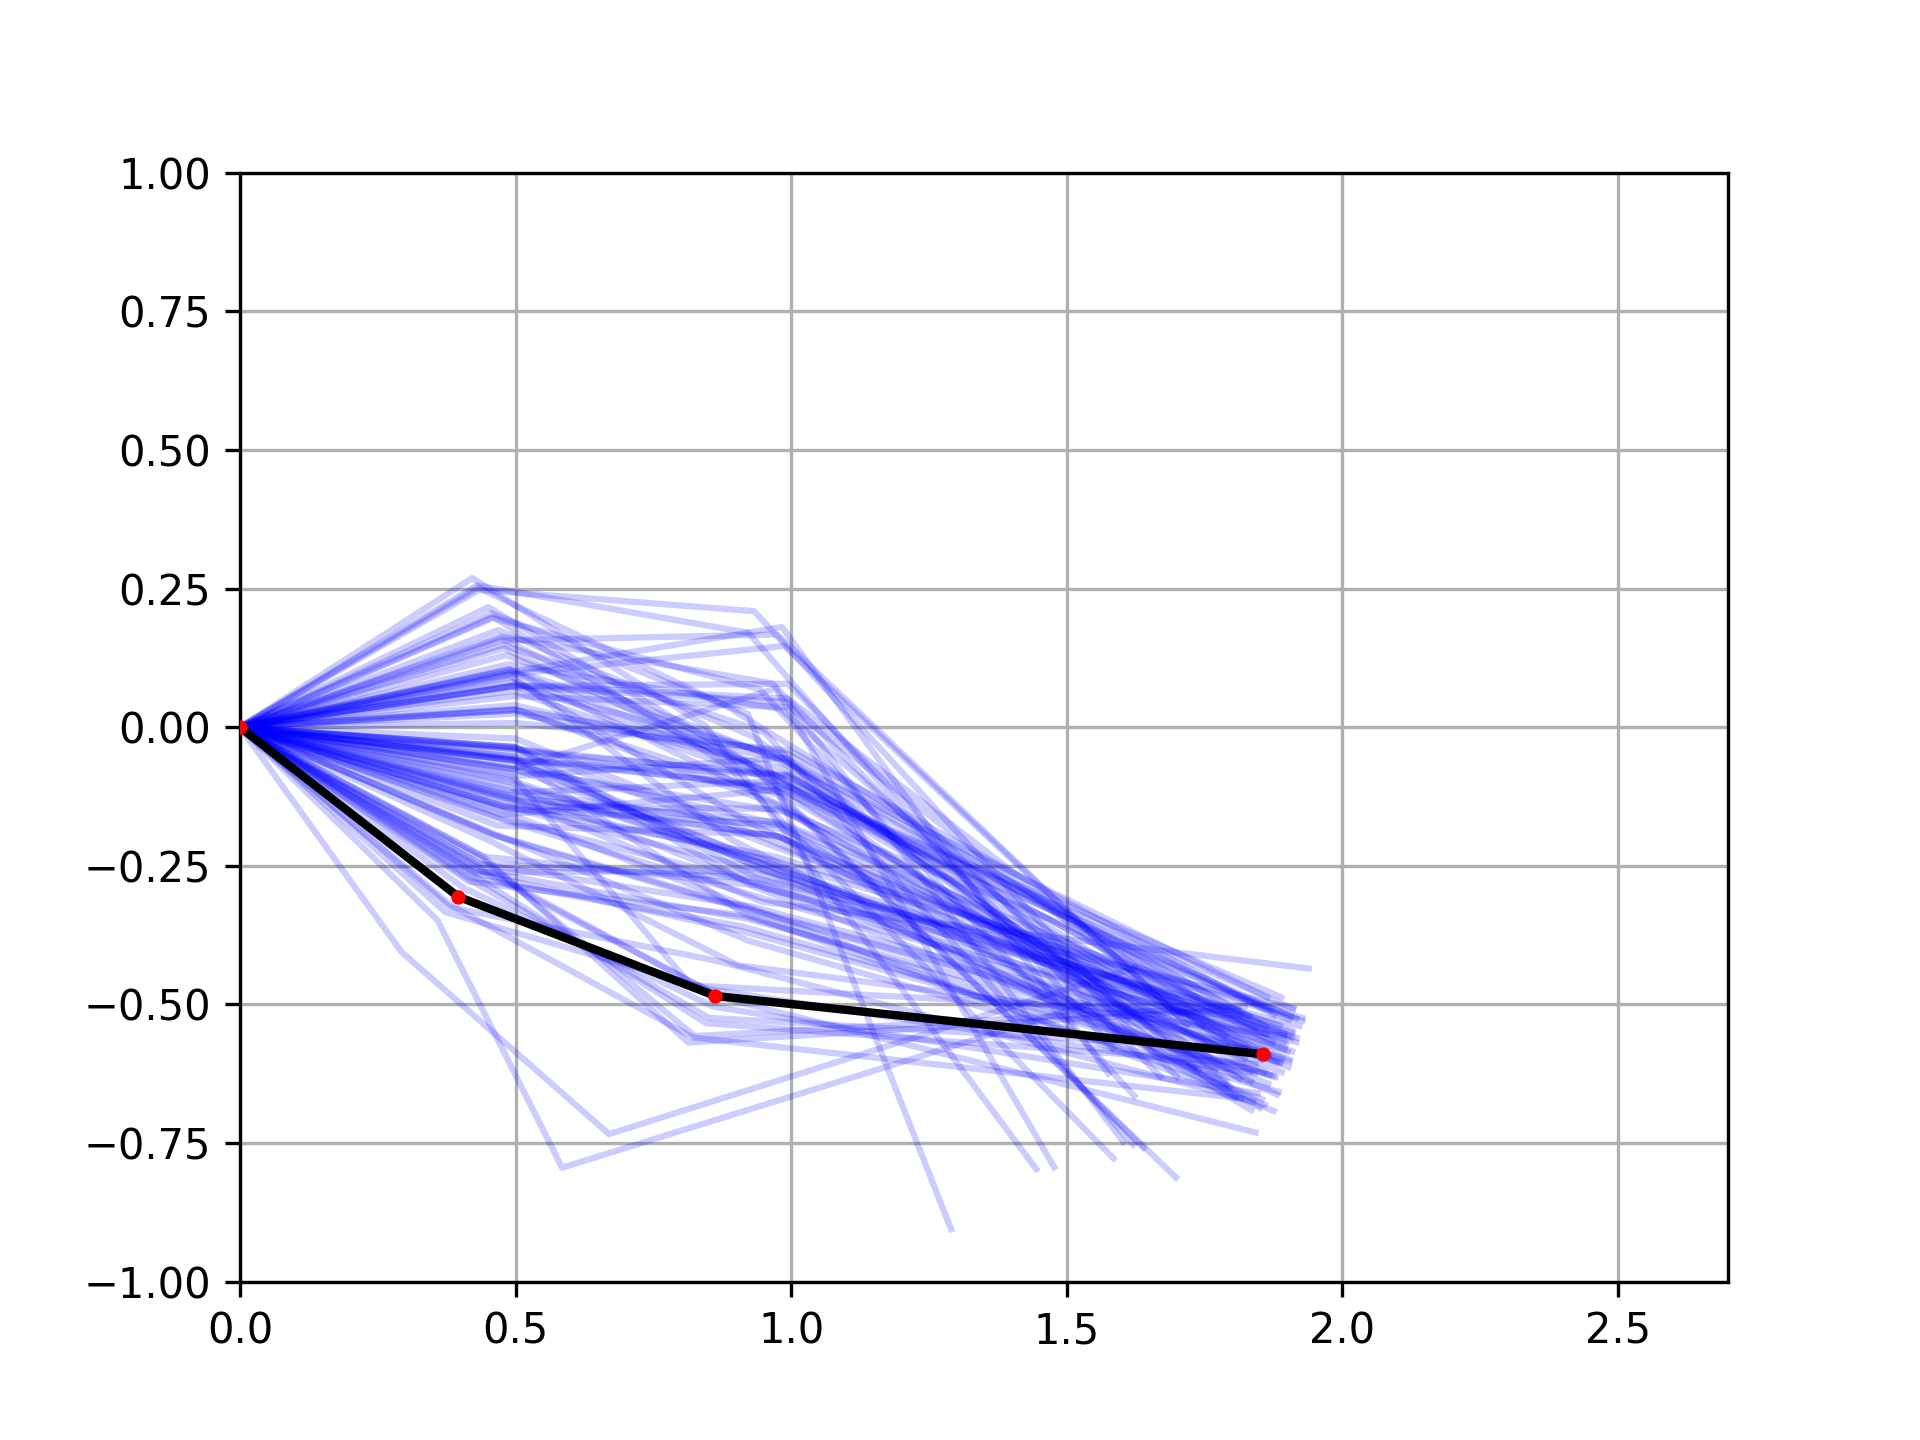
\includegraphics[width=0.29\linewidth]{figures/predicted_posterior_INN_3DOF.png}
    \label{fig:INN:3DOF}}
    
	\caption{\label{fig:posterior:3dof} Arm configuration of a planar manipulator with 3 revolute joints and end-effector position at $(x, y) = [1.83, -0.57]$. 100 samples are drawn from each model's predicted posterior $\tilde{p}(x | y_{gt})$, one random sample configuration is highlighted.}
\end{figure*}

\begin{figure*}[t]
\centering
	\subfloat[Rejection Sampling]{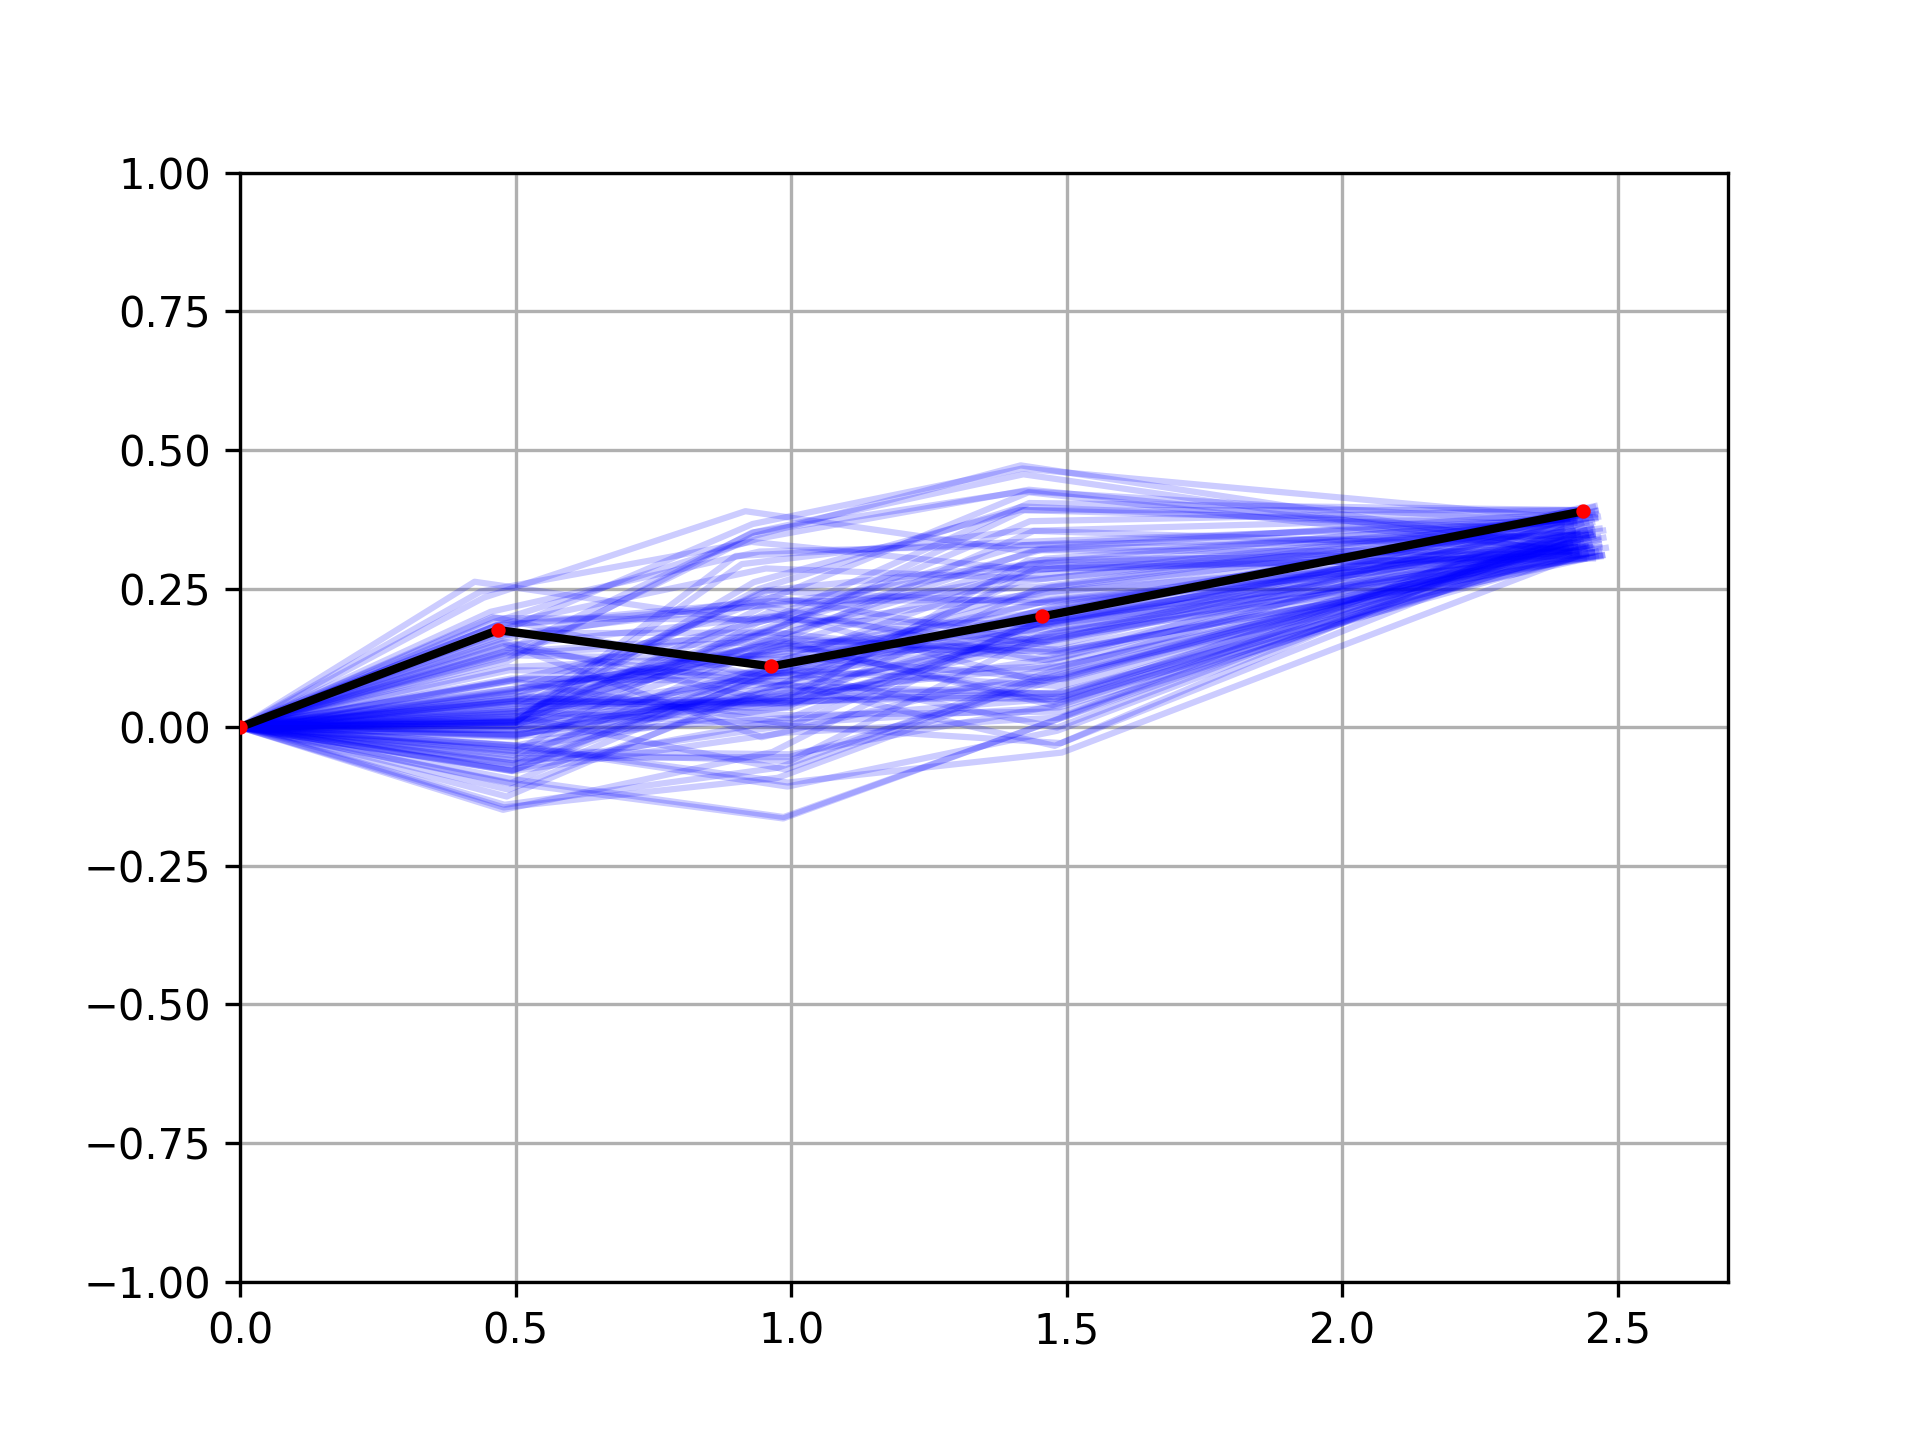
\includegraphics[width=0.29\linewidth]{figures/rejection_sampling_CVAE_4DOF.png}
    \label{fig:rejection_sampling:4DOF}}
    %
    \subfloat[cVAE]{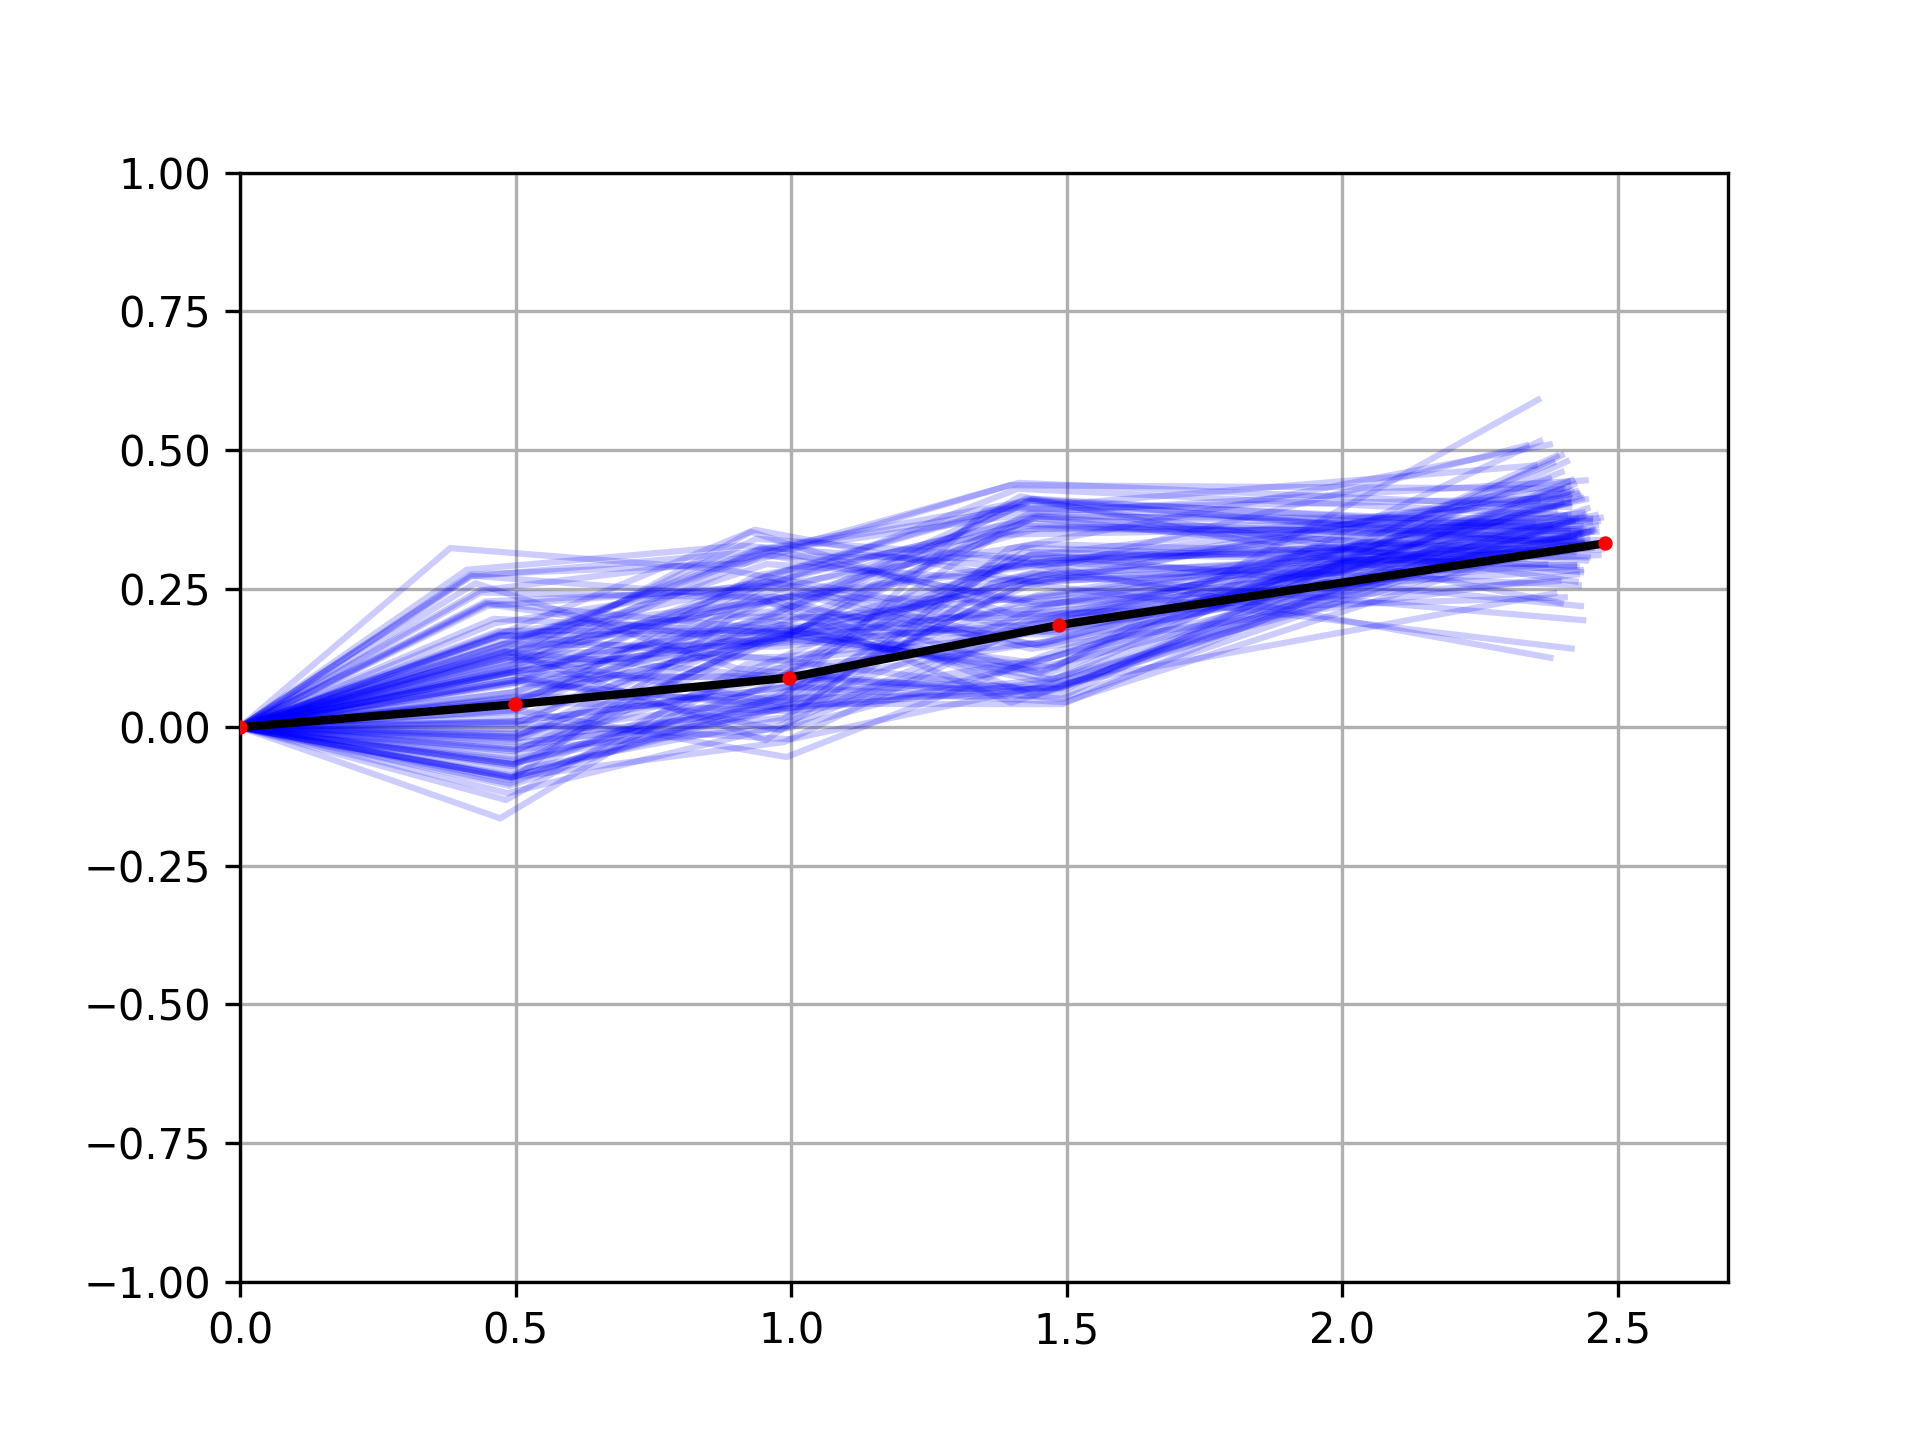
\includegraphics[width=0.29\linewidth]{figures/predicted_posterior_CVAE_4DOF.png}
    \label{fig:cVAE:4DOF}}
    %
    \subfloat[INN]{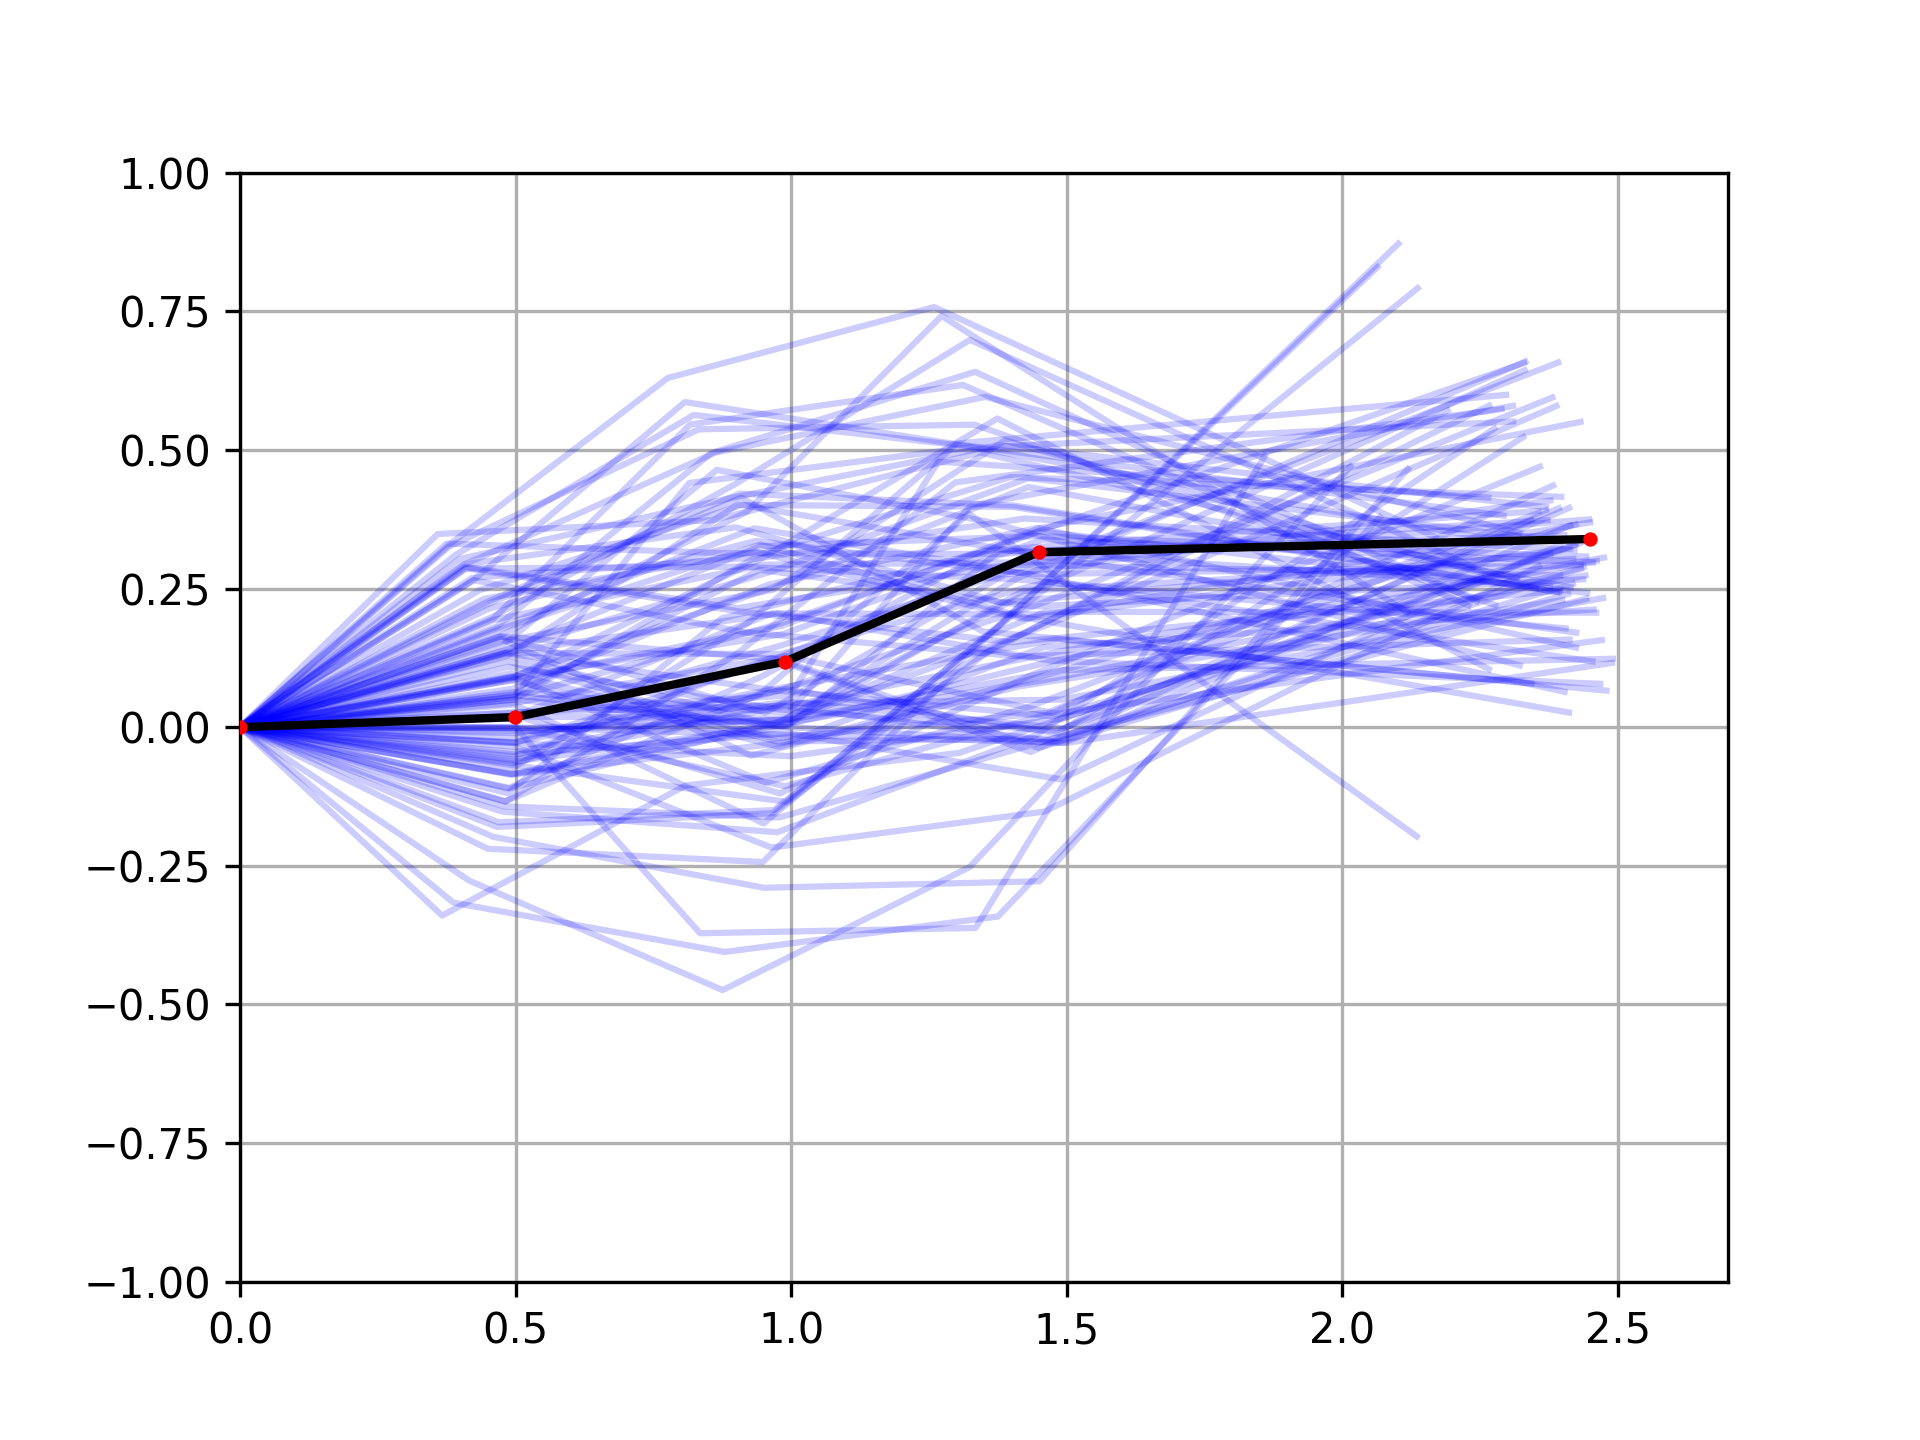
\includegraphics[width=0.29\linewidth]{figures/predicted_posterior_INN_4DOF.png}
    \label{fig:INN:4DOF}}
    
	\caption{\label{fig:posterior:4dof} Arm configuration of a planar manipulator with 4 revolute joints and end-effector position at $(x, y) = [2.44, 0.35]$. 100 samples are drawn from each model's predicted posterior $\tilde{p}(x | y_{gt})$, one random sample configuration is highlighted.}
\end{figure*}


\section*{Next Steps}


\nocite{*}
\bibliographystyle{IEEEtran}
\bibliography{IEEEabrv,midterm_report}

\end{document}
